\documentclass[11pt,aspectratio=169]{beamer}

\usepackage{booktabs}
\usepackage{array}
\usepackage{multirow}
\usepackage{tikz}
\usepackage{pgfplots}
\usepackage{xcolor}
\usepackage{amsmath}
\usepackage{mathtools}
\usepackage{listings}
\usetikzlibrary{positioning,calc,arrows.meta,decorations.pathreplacing}
\pgfplotsset{compat=1.18}

\usetheme[titleformat=smallcaps,progressbar=frametitle]{metropolis}
\definecolor{UTburnt}{HTML}{BF5700}
\definecolor{LBJnavy}{HTML}{172A46}
\definecolor{softgray}{HTML}{F2F3F5}
\definecolor{midgray}{HTML}{6B7280}
\definecolor{softorange}{HTML}{F9E7DA}
\definecolor{softgreen}{HTML}{E8F2EC}
\setbeamercolor{alerted text}{fg=UTburnt}
\setbeamercolor{frametitle}{bg=LBJnavy,fg=white}
\setbeamercolor{progress bar}{fg=UTburnt,bg=gray!25}
\setbeamercolor{block title}{bg=LBJnavy!10,fg=LBJnavy}
\setbeamercolor{block body}{bg=softgray}
\setbeamertemplate{navigation symbols}{}
\setbeamertemplate{itemize item}{\color{UTburnt}$\blacktriangleright$}
\setbeamertemplate{itemize subitem}{\color{UTburnt}$\bullet$}

\lstset{
  basicstyle=\ttfamily\scriptsize,
  backgroundcolor=\color{softgray},
  frame=single,
  rulecolor=\color{midgray!40},
  columns=fullflexible,
  keepspaces=true,
  showstringspaces=false
}

\author{Sergio I. Garc\'ia-R\'ios}
\title{Hypothesis Testing}
\subtitle{When is a sample result too unusual to dismiss as sampling variability?}
\institute{PA 311N: Data Analysis for Public Policy\\LBJ School of Public Affairs}
\date{October 19, 2026}

\newcommand{\yourturn}[1]{%
\pause
\begin{center}
\begin{minipage}{0.90\textwidth}
\begin{alertblock}{Your Turn}
#1
\end{alertblock}
\end{minipage}
\end{center}}

\newcommand{\ourturn}[1]{%
\pause
\begin{center}
\begin{minipage}{0.90\textwidth}
\begin{block}{Our Turn}
#1
\end{block}
\end{minipage}
\end{center}}

\newcommand{\SE}{\operatorname{SE}}

\begin{document}

% 1
\begin{frame}[plain]
\centering
\vspace{0.55cm}
{\color{LBJnavy}\LARGE\bfseries Hypothesis Testing\par}
\vspace{0.35cm}
{\large When is a sample result too unusual to dismiss as sampling variability?\par}
\vspace{0.8cm}
{\normalsize Sergio I. Garc\'ia-R\'ios\par}
\vspace{0.2cm}
{\small PA 311N: Data Analysis for Public Policy\par}
{\small LBJ School of Public Affairs\par}
\vfill
{\small October 19, 2026\par}
\end{frame}

% 2
\begin{frame}{Where we left off}
Confidence intervals asked:
\begin{center}
\Large What values of the population parameter are \alert{plausible} given our sample?
\end{center}

\vspace{0.8em}
Hypothesis tests turn the logic around:
\begin{center}
\Large Suppose a particular population value were true.\\
Would our sample result be \alert{surprising}?
\end{center}

\vfill
Same sampling-distribution logic. Different inferential question.
\end{frame}

% 3
\begin{frame}{A policy claim we can test}
The hypothetical Ames Sustainability Office plans staffing around this claim:

\begin{center}
\Large Average residential inspection time is \alert{60 minutes}.
\end{center}

A random sample of 40 inspections gives
\[
n=40,\qquad \bar{x}=66,\qquad s=18\text{ minutes}.
\]

\vfill
\begin{alertblock}{Question}
Is a six-minute difference something we could reasonably see from sampling variability alone, or is it evidence that inspections take longer than 60 minutes on average?
\end{alertblock}
\end{frame}

% 4
\begin{frame}{Two explanations for the same sample}
We observed
\[
\bar{x}=66\text{ minutes}.
\]

\begin{columns}[T,onlytextwidth]
\column{0.47\textwidth}
\begin{block}{Explanation 1}
The true mean really is 60 minutes.

Our sample happened to run high because of \alert{sampling variability}.
\end{block}
\column{0.47\textwidth}
\begin{block}{Explanation 2}
The true mean is greater than 60 minutes.

The sample is revealing a \alert{real difference} from the planning assumption.
\end{block}
\end{columns}

\vfill
Hypothesis testing asks how compatible the data are with Explanation 1.
\end{frame}

% 5
\begin{frame}[standout]
\Large Start by pretending the null claim is true.
\end{frame}

% 6
\begin{frame}{Null and alternative hypotheses}
The \alert{null hypothesis} is the benchmark claim we test:
\[
H_0:\mu=60.
\]

The \alert{alternative hypothesis} is the pattern for which we are seeking evidence:
\[
H_A:\mu>60.
\]

\vspace{0.8em}
This is a \textbf{one-sided} test because the policy concern is specifically that inspections take \emph{longer} than planned.

\vfill
\begin{block}{Important}
We do not begin by assuming $H_A$ is true. We ask whether the observed data would be unusually extreme \emph{if $H_0$ were true}.
\end{block}
\end{frame}

% 7
\begin{frame}{The alternative determines the tail}
\begin{center}
\begin{tabular}{lll}
\toprule
Policy question & Alternative & Relevant tail(s)\\
\midrule
Longer than planned? & $H_A:\mu>60$ & upper tail\\
Shorter than planned? & $H_A:\mu<60$ & lower tail\\
Different from planned? & $H_A:\mu\neq60$ & both tails\\
\bottomrule
\end{tabular}
\end{center}

\vspace{0.8em}
\yourturn{If the city only wants to know whether the average differs from 60 minutes in \emph{either direction}, what should $H_A$ be?}
\end{frame}

% 8
\begin{frame}{The logic in four steps}
\begin{enumerate}
  \item \textbf{State} $H_0$ and $H_A$.
  \item \textbf{Model} what sample statistics should look like if $H_0$ is true.
  \item \textbf{Measure} how far the observed statistic is from the null value.
  \item \textbf{Evaluate} how unusual that result would be under $H_0$.
\end{enumerate}

\vspace{1em}
That final probability is the \alert{p-value}.

\vfill
\begin{center}
\large Hypothesis testing is a structured version of:\\
\textbf{``Could random sampling reasonably have produced this?''}
\end{center}
\end{frame}

% 9
\begin{frame}{Conditions still matter}
For a one-sample $t$ test of a mean, we need the same logic that supported our confidence interval:

\begin{itemize}
  \item \textbf{Independence}: observations should come from a random process and not determine one another.
  \item \textbf{10\% condition}: if sampling without replacement, the sample should be less than about 10\% of the population.
  \item \textbf{Shape / sample size}: the population should be roughly normal, or the sample should be large enough that the sampling distribution of $\bar{x}$ is approximately normal.
\end{itemize}

\vfill
Conditions justify the reference distribution we use to calculate the p-value.
\end{frame}

% 10
\begin{frame}{How unusual is 66 if the true mean is 60?}
Under the null hypothesis,
\[
\mu_0=60.
\]

Our observed estimate is
\[
\bar{x}=66.
\]

But a six-minute difference means something different when the standard error is 1 minute versus 20 minutes.

\vfill
\begin{alertblock}{We need a standardized distance}
How many \textbf{standard errors} is the observed sample mean from the null value?
\end{alertblock}
\end{frame}

% 11
\begin{frame}{The test statistic}
For a one-sample test of a mean,
\[
\boxed{t=\frac{\bar{x}-\mu_0}{s/\sqrt{n}}}
\]

\begin{itemize}
  \item Numerator: observed difference from the null claim.
  \item Denominator: estimated standard error of the sample mean.
  \item Result: distance from the null value measured in \alert{standard errors}.
\end{itemize}

\vfill
Large $|t|$ means the sample result is far from what $H_0$ predicts.
\end{frame}

% 12
\begin{frame}{Do not confuse $t^*$ and $t$}
\begin{columns}[T,onlytextwidth]
\column{0.47\textwidth}
\begin{block}{$t^*$: critical value}
Used in a confidence interval:
\[
\bar{x}\pm t^*SE.
\]

Chosen from the desired confidence level and degrees of freedom.
\end{block}
\column{0.47\textwidth}
\begin{alertblock}{$t$: test statistic}
Calculated from the observed data:
\[
t=\frac{\bar{x}-\mu_0}{SE}.
\]

Measures how far the estimate is from the null claim.
\end{alertblock}
\end{columns}

\vfill
\alert{The star is not decoration: $t^*$ and $t$ play different roles.}
\end{frame}

% 13
\begin{frame}{Calculate the standard error}
For the inspection-time sample,
\[
n=40,\qquad s=18.
\]

So
\[
SE=\frac{s}{\sqrt{n}}
=\frac{18}{\sqrt{40}}
\approx2.85\text{ minutes}.
\]

\vfill
A sample mean from repeated samples of 40 inspections would typically vary by roughly 2.85 minutes around the true mean.
\end{frame}

% 14
\begin{frame}{Calculate the observed $t$ statistic}
Now compare the observed mean with the null value:
\[
t=\frac{66-60}{2.85}
\approx2.11.
\]

\begin{center}
\Large The sample mean is about \alert{2.11 standard errors above} the null value.
\end{center}

\vfill
Is 2.11 standard errors unusually far into the upper tail? That is exactly what the p-value answers.
\end{frame}

% 15
\begin{frame}{What would we see if $H_0$ were true?}
If $H_0:\mu=60$ is true, the test statistic follows a $t$ distribution with
\[
df=n-1=39.
\]

\begin{center}
\begin{tikzpicture}
\begin{axis}[
  width=0.83\textwidth,height=0.43\textheight,
  xmin=-4,xmax=4,ymin=0,ymax=.42,
  axis lines=middle,ytick=\empty,xtick={0,2.11},
  xticklabels={$0$,$2.11$},
  tick label style={font=\small}
]
\addplot[LBJnavy,very thick,domain=-4:4,samples=180] {0.395*exp(-x^2/2.1)};
\addplot[draw=none,fill=UTburnt!35,domain=2.11:4,samples=80] {0.395*exp(-x^2/2.1)} \closedcycle;
\draw[UTburnt,dashed,thick] (axis cs:2.11,0)--(axis cs:2.11,.14);
\node[UTburnt,font=\small,align=center] at (axis cs:2.85,.09) {results at least\\this high};
\end{axis}
\end{tikzpicture}
\end{center}

For our one-sided alternative, the p-value is the \alert{upper-tail area beyond $t=2.11$}.
\end{frame}

% 16
\begin{frame}{The p-value}
\begin{alertblock}{Definition}
The p-value is the probability of observing a result at least as extreme as ours, in the direction specified by $H_A$, \textbf{assuming the null hypothesis is true}.
\end{alertblock}

For this example:
\[
p=P(T_{39}\ge2.11)\approx0.021.
\]

\vfill
Interpretation:

If the true average inspection time were really 60 minutes, only about \alert{2.1\%} of random samples like ours would produce a sample mean this high or higher.
\end{frame}

% 17
\begin{frame}[fragile]{Calculate the p-value in R}
\begin{lstlisting}[language=R]
n <- 40
x_bar <- 66
mu_0 <- 60
s <- 18

se <- s / sqrt(n)
t_obs <- (x_bar - mu_0) / se

pt(t_obs, df = n - 1, lower.tail = FALSE)
\end{lstlisting}

\[
p\approx0.0207.
\]

\vfill
\alert{`lower.tail = FALSE' asks R for the upper-tail probability.}
\end{frame}

% 18
\begin{frame}{From evidence to a decision rule}
A p-value is continuous evidence. For a formal decision, we choose a significance level $\alpha$.

Commonly,
\[
\alpha=0.05.
\]

Decision rule:
\begin{itemize}
  \item If $p<\alpha$: \alert{reject $H_0$}.
  \item If $p\ge\alpha$: \alert{fail to reject $H_0$}.
\end{itemize}

For our example:
\[
0.0207<0.05.
\]

So we reject $H_0$ at the 5\% significance level.
\end{frame}

% 19
\begin{frame}{Interpret the decision in policy language}
Do not stop at ``reject $H_0$.''

\begin{block}{Weak conclusion}
$p<0.05$, therefore reject the null.
\end{block}

\begin{alertblock}{Policy conclusion}
The sample provides statistically significant evidence that the average residential inspection time exceeds 60 minutes.
\end{alertblock}

\vfill
This does \textbf{not} prove the true mean is exactly 66 minutes. It says the 60-minute planning assumption is difficult to reconcile with the observed sample.
\end{frame}

% 20
\begin{frame}{Fail to reject is not accept}
Suppose instead we had found
\[
p=0.32.
\]

The correct conclusion would be:

\begin{center}
\Large The sample does \alert{not provide sufficient evidence} that $\mu>60$.
\end{center}

Not:
\begin{center}
\Large ``We proved that $\mu=60$.''
\end{center}

\vfill
A non-small p-value can reflect a true null, a small effect, noisy data, or insufficient sample size.
\end{frame}

% 21
\begin{frame}{What a p-value is \emph{not}}
A p-value is \textbf{not}:

\begin{itemize}
  \item the probability that $H_0$ is true;
  \item the probability that the result happened ``by chance'';
  \item the size or practical importance of an effect;
  \item the probability that our conclusion is wrong.
\end{itemize}

\vfill
It is a conditional probability:
\[
P(\text{data as or more extreme than observed}\mid H_0\text{ true}).
\]
\end{frame}

% 22
\begin{frame}{Your turn: interpret the p-value}
\yourturn{For the Ames inspection example, $p\approx0.021$. Which interpretation is best?}

\begin{enumerate}
  \item There is a 2.1\% chance that the true mean is 60.
  \item There is a 2.1\% chance that our sample is wrong.
  \item If the true mean were 60, a sample result this high or higher would occur about 2.1\% of the time.
  \item About 2.1\% of inspections take more than 60 minutes.
\end{enumerate}

\pause
\begin{center}
\alert{Best answer: (3). The probability is calculated assuming $H_0$ is true.}
\end{center}
\end{frame}

% 23
\begin{frame}{One-sided versus two-sided p-values}
Our original question was directional:
\[
H_A:\mu>60.
\]
so we used only the upper tail:
\[
p_{\text{one-sided}}\approx0.021.
\]

If instead
\[
H_A:\mu\ne60,
\]
then equally extreme deviations in \emph{either direction} count:
\[
p_{\text{two-sided}}\approx2(0.021)=0.041.
\]

\vfill
Choose the alternative from the substantive question, \alert{not after seeing the data}.
\end{frame}

% 24
\begin{frame}{Confidence intervals and two-sided tests agree}
\small
Using the same sample,
\[
\bar{x}=66,\quad SE\approx2.85,\quad df=39.
\]

The 95\% confidence interval is approximately
\[
66\pm2.023(2.85)
=(60.24,\,71.76).
\]

The null value 60 is \alert{outside} the 95\% interval.

\vspace{0.35em}
That matches the two-sided test:
\[
p\approx0.041<0.05.
\]

\begin{block}{Connection}
A two-sided test at $\alpha=0.05$ rejects exactly those null values excluded by the corresponding 95\% confidence interval.
\end{block}
\end{frame}

% 25
\begin{frame}{What does $\alpha=0.05$ mean?}
The significance level controls how willing we are to reject $H_0$ when it is actually true.

\begin{center}
\Large $\alpha=0.05$ sets a \alert{5\% Type I error rate} under repeated testing.
\end{center}

\vspace{0.8em}
It is a decision threshold chosen \emph{before} looking at the result.

\vfill
Smaller $\alpha$ requires stronger evidence to reject $H_0$.
\end{frame}

% 26
\begin{frame}{Two ways a decision can be wrong}
\begin{center}
\begin{tabular}{llcc}
\toprule
& & \multicolumn{2}{c}{\textbf{Decision}}\\
& & Fail to reject $H_0$ & Reject $H_0$\\
\midrule
\multirow{2}{*}{\textbf{Truth}} & $H_0$ true & Correct & \alert{Type I error}\\
& $H_A$ true & \alert{Type II error} & Correct\\
\bottomrule
\end{tabular}
\end{center}

\vspace{1em}
\begin{itemize}
  \item Type I: false positive.
  \item Type II: false negative.
\end{itemize}

\vfill
There is no decision rule that eliminates both errors in every sample.
\end{frame}

% 27
\begin{frame}{Type I error in the inspection example}
Recall:
\[
H_0:\mu=60,\qquad H_A:\mu>60.
\]

A \alert{Type I error} would mean:

\begin{center}
\Large Concluding that inspections take longer than 60 minutes on average\\
when the true mean is actually 60.
\end{center}

\vfill
Possible policy consequence: the city expands staffing or budgets additional time when that change was not actually necessary.
\end{frame}

% 28
\begin{frame}{Type II error in the inspection example}
A \alert{Type II error} would mean:

\begin{center}
\Large Failing to detect that inspections really do take longer than 60 minutes on average.
\end{center}

\vfill
Possible policy consequence: the city keeps an unrealistic staffing model, causing delays, overtime, or missed appointments.

\vspace{0.8em}
\yourturn{Which error would be more costly in this policy setting? What information would you need to decide?}
\end{frame}

% 29
\begin{frame}{Power: the ability to detect a real effect}
\alert{Power} is the probability that a test correctly rejects $H_0$ when a meaningful alternative is true.

Power generally increases when:
\begin{itemize}
  \item the true effect is larger;
  \item the sample size is larger;
  \item the data are less variable;
  \item we use a less stringent $\alpha$.
\end{itemize}

\vfill
A study can fail to find statistical significance simply because it had too little information to detect the effect reliably.
\end{frame}

% 30
\begin{frame}{Statistical significance is not policy significance}
Suppose a huge study estimates that a new scheduling system changes average wait time by
\[
0.4\text{ minutes}
\]
with
\[
p<0.001.
\]

The result is statistically distinguishable from zero.

But is a 24-second improvement worth implementation costs?

\vfill
\begin{alertblock}{Two separate questions}
Is the effect statistically detectable?\\
Is the effect substantively important for the policy decision?
\end{alertblock}
\end{frame}

% 31
\begin{frame}{A hypothesis test is not a verdict machine}
A good policy analysis reports more than ``significant'' or ``not significant.''

Report:
\begin{itemize}
  \item the estimate and its units;
  \item uncertainty, preferably a confidence interval;
  \item the test statistic and p-value when relevant;
  \item the size and practical meaning of the effect;
  \item assumptions and design limitations.
\end{itemize}

\vfill
\alert{Evidence informs a decision. It does not make the decision for us.}
\end{frame}

% 32
\begin{frame}{The full workflow}
\begin{enumerate}
  \item \textbf{Question}: what policy claim are we evaluating?
  \item \textbf{Hypotheses}: state $H_0$ and $H_A$.
  \item \textbf{Conditions}: is the inferential model defensible?
  \item \textbf{Estimate uncertainty}: $SE=s/\sqrt{n}$.
  \item \textbf{Standardize}: $t=(\bar{x}-\mu_0)/SE$.
  \item \textbf{Tail probability}: calculate the p-value.
  \item \textbf{Decision}: compare p with $\alpha$ if a formal rule is needed.
  \item \textbf{Interpret}: translate the evidence into policy language.
\end{enumerate}
\end{frame}

% 33
\begin{frame}{Your turn: set up the test}
A city claims the average permit-processing time is 30 days. A random sample suggests the process may be slower.

\yourturn{Write the hypotheses for a test of whether the true mean processing time exceeds 30 days.}

\vspace{0.8em}
\ourturn{
\[
H_0:\mu=30
\qquad\text{vs.}\qquad
H_A:\mu>30.
\]
The relevant p-value will be an \textbf{upper-tail} probability.}
\end{frame}

% 34
\begin{frame}{What to remember}
\begin{itemize}
  \item Hypothesis tests ask whether the observed data are compatible with a specific null claim.
  \item The test statistic measures distance from the null value in \alert{standard errors}.
  \item The p-value asks how unusual the observed result would be \alert{if $H_0$ were true}.
  \item Reject $H_0$ when evidence is sufficiently inconsistent with it; otherwise \alert{fail to reject}.
  \item Statistical significance is not the same as practical importance.
\end{itemize}

\end{frame}

% 35
\begin{frame}[standout]
\Large The p-value is not the probability\\that the null is true.\\[0.7em]
\normalsize It is a measure of how surprising the data would be if the null were true.
\end{frame}

\end{document}